%% https://github.com/tbielawa/PAD-XMPP/blob/master/Graph/ConnectionStates.png
\documentclass{article}
\usepackage{fullpage}
\usepackage{booktabs}
\usepackage{amsmath}
\usepackage{amssymb}
\usepackage[noend]{algorithmic}
\usepackage[nothing]{algorithm}
\usepackage{tikz}
\usepackage{latexsym}
\usepackage{float}
\usepackage{hyperref}
\usetikzlibrary{arrows,automata}
\providecommand{\e}[1]{\ensuremath{\times 10^{#1}}}
\renewcommand{\thealgorithm}{}
\renewcommand*{\thefootnote}{[\arabic{footnote}]}
\title{CS 544: Computer Networks \\ Term Paper I -- XMPP Protocol Analysis}
\author{Dustin Ingram}
\begin{document}
\maketitle
\section{Background}
The Extensible Messaging and Presence Protocol (XMPP) is a stateful
application layer protocol primarily used for instant-messaging (IM). XMPP was
initially conceived as the open-source Jabber messaging protocol by Jeremie
Miller in 1998
\footnote{\url{http://xmpp.org/about-xmpp/xsf/xsf-people/\#bdfl}}, after which
it was extensively developed the open-source developer community which
surrounded it. In 2002, the Internet Engineering Task Force (IETF) approved the
creation of the XMPP Working Group to focus on refining the protocol into an
IETF standard.\footnote{\url{http://xmpp.org/about-xmpp/history/}}

\subsection{XMPP and related IETF RFCs}
The IETF's XMPP Working Group and it's successor, the XMPP Standards Foundation,
have produced a number of RFCs related to
XMPP.\footnote{\url{http://xmpp.org/xmpp-protocols/rfcs/}}

\subsubsection{RFC 2778 and RFC 2779}
The informational RFCs \emph{``A Model for Presence and Instant Messaging''}
(RFC 2778) and \emph{``Instant Messaging / Presence Protocol Requirements''}
(RFC 2779) were published in 2000 by the IETF Instant Messaging and Presence
Protocol (IMPP) Working Group. These were produced in parallel with the work
being done by the Jabber community at the time, and pre-date the existence of
the XMPP Working Group. 

\subsection{RFC 3920 and RFC 3921}
These RFCs, \emph{``XMPP: Core''} and \emph{``XMPP: Instant Messaging and
Presence''}, were the first RFCs produced by the XMPP Working Group which were
accepted by the IETF in 2004 as conforming to the standards set by RFC 2778 and
RFC 2779, and essentially defined XMPP v1.0.

\subsection{RFC 6120 and RFC 6121}
These RFCs obsolete RFC 3920 and RFC 3921, respectively, and are based on over
six years of feedback between RFCs from the XMPP developer community, and the
XMPP Standards Foundation (XSF). A number of important issues that existed in
the previous iteration of these RFCs are addressed in the latest versions.

\subsection{Other RFCs}
\begin{itemize}
    \item \textbf{RFC 3922} -- Mapping the Extensible Messaging and Presence
        Protocol (XMPP) to Common Presence and Instant Messaging (CPIM)
    \item \textbf{RFC 3923} -- End-to-End Signing and Object Encryption for the
        Extensible Messaging and Presence Protocol (XMPP)
    \item \textbf{RFC 4854} -- A Uniform Resource Name (URN) Namespace for
        Extensions to the Extensible Messaging and Presence Protocol (XMPP)
    \item \textbf{RFC 4979} -- IANA Registration for Enumservice `XMPP'
    \item \textbf{RFC 5122} -- Internationalized Resource Identifiers (IRIs) and
        Uniform Resource Identifiers (URIs) for the Extensible Messaging and
        Presence Protocol (XMPP)
    \item \textbf{RFC 6122} -- Extensible Messaging and Presence Protocol
        (XMPP): Address Format
\end{itemize}

\subsection{Scope of this Analysis}
Since the XMPP protocol consists of a number of related RFCs which provide
different areas of functionality, this paper will focus solely on the core of
the protocol, RFC 6120, \emph{``XMPP: Core''}. Furthermore, since RFC 6120
provides information for Client-to-Server as well as Server-to-Server
implementations of the XMPP protocol, the focus of this analysis will
additionally restrict itself to only the Client-to-Server portion of the
protocol, as it is arguably more widely used.

\section{Services Provided by the XMPP Protocol}
The core of the XMPP Protocol seeks to provide asynchronous application-layer
instant-messaging (IM) and information exchange. This mainly involves the
transfer of transfer of small, text-only (non-binary) messages, although
extensions exist for file transfers, amongst other things. The typical
implementation and use of the XMPP protocol is in a Client-to-Server scenario,
however, RFC 6120 also provides a reference for Server-to-Server communication,
in the case of server federation and inter-communication. The combination of
these two typical scenarios produces a ``distributed client-server
architecture'', where multiple clients can interoperate through a network of
multiple servers.

\section{Overview of XMPP Communication Architecture}
\subsection{Messaging Architecture}
In a general sense, XMPP uses a structured message format similar to XML, which
the protocol calls ``XML stanzas'' or just ``stanzas'', for all information
exchange. The main difference between a ``stanza'' and an XML file is that
stanzas may not (and often are not) complete XML documents in the typical sense,
as XMPP uses the notion of these individual chunks of XML-esque information to
``stream'' information, starting connections with an opening tag and ending them
with a closing tag, and over the course of one connection and information
exchange, building a complete document. 

The XMPP protocol uses three types of XMPP stanzas, essentially XML element
tags, to denote different types of messaging. They include:

\begin{itemize}
    \item ``Messages'', using the \texttt{<message>} tag
    \item ``Presence Messages'', using the \texttt{<presence>} tag
    \item ``IQ Messages'', using the \texttt{<iq>} tag
\end{itemize}

Each of these message types are discussed at length in subsequent sections.

\subsubsection{Issues with the Messaging Architecture}
The XMPP stanza structure can present problems when it comes to implementing
clients or servers, as most standard libraries for XML parsing require a
complete document, otherwise they are unable to parse. Since XMPP stanzas are,
by definition, incomplete fragments of an XML document, this often requires the
use of unique, underused or custom XML parsers to use the raw transmitted
information in a meaningful way.

Furthermore, XMPP's reliance on XML-based message structure is a hallmark and
indicator of it's age. While XML is useful as a human-readable markup language,
that feature is not necessarily a requirement within the XMPP protocol, where
messages are abstracted and hidden by client and server implementations.  

As a result, XML is generally considered to be a unnecessarily verbose language
format. In relation to XMPP, this may be undesirable in instances where
bandwidth is constrained or the network is congested.

\subsection{Addressing Scheme}
Addressing is inherent to the XMPP protocol -- so much so, in fact, that there
is an entire published RFC specifically for the XMPP address format. However,
the addressing scheme necessary to understand the XMPP Core Protocol is simple
enough to be described succinctly. 

XMPP addresses, also known as ``Jabber IDs'' or ``JIDs'', have the following
general structure:
\begin{center}
$\underbrace{\texttt{client}}_\text{local
part}\texttt{@}\underbrace{\texttt{chat.example.com}}_\text{domain
part}\texttt{/}\underbrace{\texttt{nickname}}_\text{resource part}$
\end{center}

The XMPP protocol is designed to use these addresses to route messages to any
globally accessible server, as the ``domain part'' will represent a globally
unique address based on the DNS standard. The ``local part'' represents an
individual user's account at any given domain -- which may or may not represent
a single server, as domains may be spread between multiple servers. The
``resource part'' simply identifies a ``nickname'' or ``alias'' for the user in
instances where one might be necessary, such as multi-user chat.

\subsubsection{Issues with the Addressing Scheme}
This addressing scheme works well on the Internet, where domains are regulated
and unique, but such a reliance on DNS can pose issues on a network without a
need for domains or the DNS protocol. Often, in a situation where the network is
isolated from the Internet, this would require a custom DNS solution or manual
hostname organization.

Furthermore, dependence on DNS for the resolution of domain names simply means
that the XMPP protocol depends directly on the DNS protocol, and therefore
inherits and possesses all the issues and hardships that come with it.

\section{Overview of XMPP Communication Primitives}
As mentioned in the previous section, the XMPP protocol defines the basic
communication primitive of the protocol to be the XMPP stanzas. There are three
individual first-level elements which are considered proper XMPP stanzas.

\subsection{Messaging}
The ``Message'' primitive provides a simple `push' mechanism, whereby a
\texttt{<message>} stanza is sent with a payload between the start and end tags
of the stanza. Here, the payload can be nearly anything, as specified by the
various possible extensions to the protocol, but is most often a plain-text
message, or more recently common, an HTML message.

\subsection{Network Availability (`Presence')}
The ``Presence'' primitive provides a Broadcast or Publish/Subscribe service for
a XMPP client to advertise it's ``network availability''. This is identical to
the notion of online/offline status many IM networks employ, however XMPP
Presence is particularly extendable as it can describe virtually any type of
status or presence message by design.

The XMPP protocol further provides a specification to give servers the ability
to support presence subscriptions, whereby one client can `subscribe' to the
presence of another client. This is further defined in RFC 6121. 

\subsection{Request-Response Interactions (`IQ')}
The ``IQ'' or Info/Query communication primitive provides a simple request \&
response mechanism. The RFC accurately relates this to the Hypertext Transfer
Protocol (HTTP) as it has similar query `types'; the XMPP protocol uses
\texttt{GET}, \texttt{SET}, \texttt{RESULT}, and \texttt{ERROR} as it's IQ ID
types.

\subsubsection{Alternatives to XMPP IQ for Info/Query}
The RFC portrays XMPP's IQ primitive as a similar, yet distinctly different
protocol compared to HTTP. However, this RFC was written at a time when HTTP was
not being used nearly as much as a stateful protocol as it is today. With the
advent of RESTful API's and REST styled HTTP architectures, it may be possible
to replace the IQ stanza entirely with a more adaptive and descriptive
primitive.

\subsection{Other First-Level Elements}
There are a number of first-level elements which may occur in an XMPP stream
which are not considered XMPP stanzas. These may include self-closing stanza
elements, elements without a qualified Jabber namespace, or feature negotiation
elements.

\section{States of the Protocol}
A simple state diagram, showing basic connection and initialization of the XMPP
protocol. Here, $q5$ is the only state in which the protocol accepts and
transmits messages. However, this is most likely the state the protocol spends
the most time in, and this this state alone contains the bulk of the additional
portions of the protocol.

Producing an error in any state always results in a transition to the
disconnected state, $q7$, so these transitions are not shown.

        \begin{figure}[!h]
            \centering
            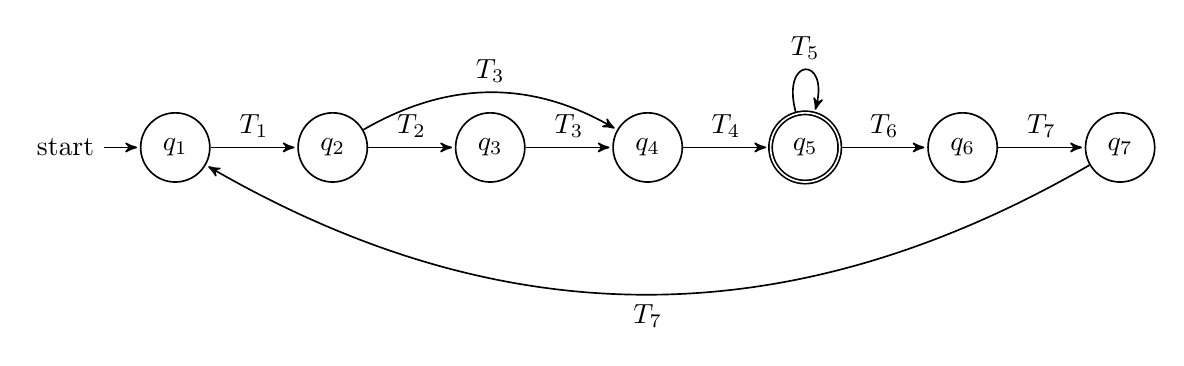
\begin{tikzpicture}[->,>=stealth',shorten >=1pt,auto,node distance=2.8cm,semithick]
              \node[state, initial]     (q1) at (0,0)  {$q_{1}$};
              \node[state]     (q2) at (2,0)  {$q_{2}$};
              \node[state]     (q3) at (4,0) {$q_{3}$};
              \node[state]     (q4) at (6,0) {$q_{4}$};
              \node[state, accepting]     (q5) at (8,0) {$q_{5}$};
              \node[state]     (q6) at (10,0) {$q_{6}$};
              \node[state]     (q7) at (12,0) {$q_{7}$};

              \path (q1) edge node {$T_{1}$} (q2)
                    (q2) edge node {$T_{2}$} (q3)
                    (q2) edge[bend left] node {$T_{3}$} (q4)
                    (q3) edge node {$T_{3}$} (q4)
                    (q4) edge node {$T_{4}$} (q5)
                    (q5) edge[loop above] node {$T_{5}$} (q5)
                    (q5) edge node {$T_{6}$} (q6)
                    (q6) edge node {$T_{7}$} (q7)
                    (q7) edge[bend left] node {$T_{7}$} (q1);
            \end{tikzpicture}
        \end{figure}
\begin{itemize}
    \item start -- Open a TCP connection
    \item $T_{1}$ -- Open an XML Stream over TCP
    \item $T_{2}$ -- Negotiate TLS for channel encryption (optional)
    \item $T_{3}$ -- Authenticate using a SASL mechanism
    \item $T_{4}$ -- Bind a resource to a stream
    \item $T_{5}$ -- Exchange an unbounded amount of XML stanzas
    \item $T_{6}$ -- Close the XML Stream (with a \texttt{</stanza>}) 
    \item $T_{7}$ -- Close the TCP connection 
    \item $T_{8}$ -- Open a new TCP connection 
\end{itemize}
\subsection{Connection Initialization}
The XMPP protocol uses a pair of persistent TCP connections for each
Client-to-Server or Server-to-Server to provide what the RFC describes as an
``always-on'' stream which allows any entity to immediately push data to any
other connected entity.

\subsubsection{Reconnection and Reliability}
The XMPP protocol provides an interesting feature to avoid massive synchronized
reconnection. Essentially, in the case of a server disconnection (thus severing
the TCP connection), to avoid what may be a large number of clients from
immediately trying to re-connect to the server at once, the protocol specifies
that clients should wait to reconnect for an ``unpredictable number between 0
and 60'' seconds, and then ``back off increasingly between subsequent
reconnection attempts''.

This essentially manages congestion of the server by reducing the load at any
given second to one sixtieth of the load it would have been previously handling,
and is a simple and elegant solution to the problem.

The RFC addresses reliability of ``long-lived TCP connections in XMPP'' as being
inherently unreliable, as they ``might not discover a connectivity disruption in
a timely manner''. The reasons for this are beyond the scope of this analysis,
but the protocol attempts to overcome this by introducing an extension outside
the core protocol.

\subsubsection{Issues with TCP as the UTM}
While using TCP as the underlying transport mechanism is clearly necessary to
enable immediate routing and provide truly \emph{instantaneous} messaging, there
are a few known issues that might manifest themselves in certain use cases.

As previously mentioned with the issues with XML, TCP is also a verbose
protocol, and may be non-ideal or even unacceptable for constrained networks.
Also as previously mentioned, long-lived TCP connections lend themselves to
being unreliable, a condition which is not immediately repairable by either
protocol.

Furthermore, in certain situations, the XMPP protocol may be using TCP too
heavily in cases where other protocols may be optimal. For example, when a
number of clients are communicating in a multi-user chat (MUC) room, each
individual client maintains a TCP connection to the server, and vice versa. The
server, then, takes on the responsibility of routing and distributing messages
through each TCP connection to the intended client. In most cases, though, all
clients in the MUC are the intended clients, and the extra bandwidth (sending
the same TCP message over a different connection for every client) can be
avoided.

\section{Authentication}
The XMPP protocol uses the Simple Authentication and Security Layer (SASL)
exclusively to provide ``a reliable mechanism for peer entity authentication''.
Therefore, every client and server implementation \emph{must} implement SASL.
SASL is a protocol within it's own right, and likely doesn't need further
description within the context of the XMPP protocol, as XMPP core uses it in a
relatively standard way.

\section{Security (Channel Encryption)}
The XMPP protocol uses a specific extension of the Transport Layer Security
(TLS) protocol and certification to encrypt and secure the stream and to
establish trust by verifying trusted entities. Similar to SASL, the protocol
requires that all client and server implementations support TLS -- however,
actual use of TLS is left to the user to decide, and thus is not mandatory.

\section{XMPP Extension Protocols}
XMPP is inherently extendable -- after all, it's in the name. Within the XMPP
protocol lies a number of XMPP Extension Protocols, otherwise known as XEPs,
which provide additional functionality across a wide range of applications on
top of the core protocol. For example, XEP-0045 defines an extension for
multi-user chat, which builds upon this RFC in the same way that this RFC builds
upon other standards.

\section{Conclusion}
To conclude, I find that XMPP is a robust and highly extendable protocol. It is
specifically designed to be adaptable and have a multitude of swappable
sub-protocols to make it applicable for a variety of scenarios, through the
existence of the XEPs to the XMPP Standards Foundation itself. 

The protocol has few weaknesses, if any. Specifically, the protocol is designed
to operate on a high-bandwidth enterprise network, and likely will not perform
well on a mobile, high-latency, low-bandwith network without significant
modification.

Furthermore, certain components, such as the IQ stanzas, may be better served by
relatively young technologies emerging from the evolution of the Internet since
the protocols first inception.
\end{document}
